\documentclass[10pt]{article}
\usepackage[margin=1in]{geometry}
 \usepackage{auto-pst-pdf}
\usepackage{graphicx}
%\usepackage{arydshln}
\usepackage{ifpdf}
\ifpdf
  \usepackage{epstopdf}
\fi
\usepackage{multirow}
\usepackage{epsfig}
\usepackage{float}
\usepackage{url}
\usepackage{color}
\usepackage{subfigure}

%\newcommand\solidrule[1][1cm]{\rule[0.5ex]{#1}{.4pt}}
%\newcommand\dashedrule{\mbox{%
%  \solidrule[2mm]\hspace{2mm}\solidrule[2mm]\hspace{2mm}\solidrule[2mm]}}
  
%\usepackage{hyperref}

\begin{document}
\title{A Study of Experiment Repeatability}

\author{
Young-Kyoon Suh\\
}
\maketitle

\section{Description}
This document presents histograms rendered based on empirical data 
of a program under test, called {\em INC}. 
Our experiment increases a task length of {\em INC} 
from one second to 4096 seconds by a factor of two.
We already ran this experiment last month (February 2017), 
but we reran the experiment this month (March 2017) 
to check if experiment repeatability holds true.

\section{Experiment Notes}
Table~\ref{tab:exp_notes} provides a short description of our experimental runs, 
on which the following histograms are based.

%% done
\begin{table}[h]
\begin{center}
\begin{tabular}{|p{2cm}|p{3cm}|p{6cm}|p{4cm}|} \hline
Machine & Task Length (sec) & Description & Experiment Period\\ \hline
{\tt sodb9} &  INC1$\sim$INC512 & Each run with 1000 samples & 2017-03-02 $\sim$ 2017-03-07\\ \hline
%{\tt sodb10} & INC2048 & A run of 300 samples & 2017-02-12 $\sim$ 2017-02-20\\ \hline
%{\tt sodb12} & INC4096 & A run of 300 samples & 2017-02-12 $\sim$ 2017-02-27\\ \hline
%{\tt sodb12} & INC8192 & Two runs, each with 40 samples & 2017-01-16 $\sim$ 2017-01-20 / 2017-01-25 $\sim$ 2017-01-29\\ \hline
%{\tt sodb12} & INC16384 & Two runs, each with 40 samples & 2017-01-05 $\sim$ 2017-01-13 / 2017-01-29 $\sim$ 2017-02-06\\ \hline 
\end{tabular}
\end{center}
\vspace{-.2in}
\caption{Notes on experiment runs used for histograms\label{tab:exp_notes}}
\end{table}

Now we show histograms of elapsed time (ET) and process time (PT) of INC. 

\newpage

\newpage

\subsection{{\tt sodb12}~\label{sec:sodb12_hist}} 
This section exhibits histograms on the EMPv5 data obtained on {\tt sodb12}. 
The detailed description of the base data are from Table~\ref{tab:exp_notes}.

\subsubsection{ET}

\begin{figure}[hp!]
	\centering
	\subfigure[ET frequency on INC1 on {\tt sodb12}]{
		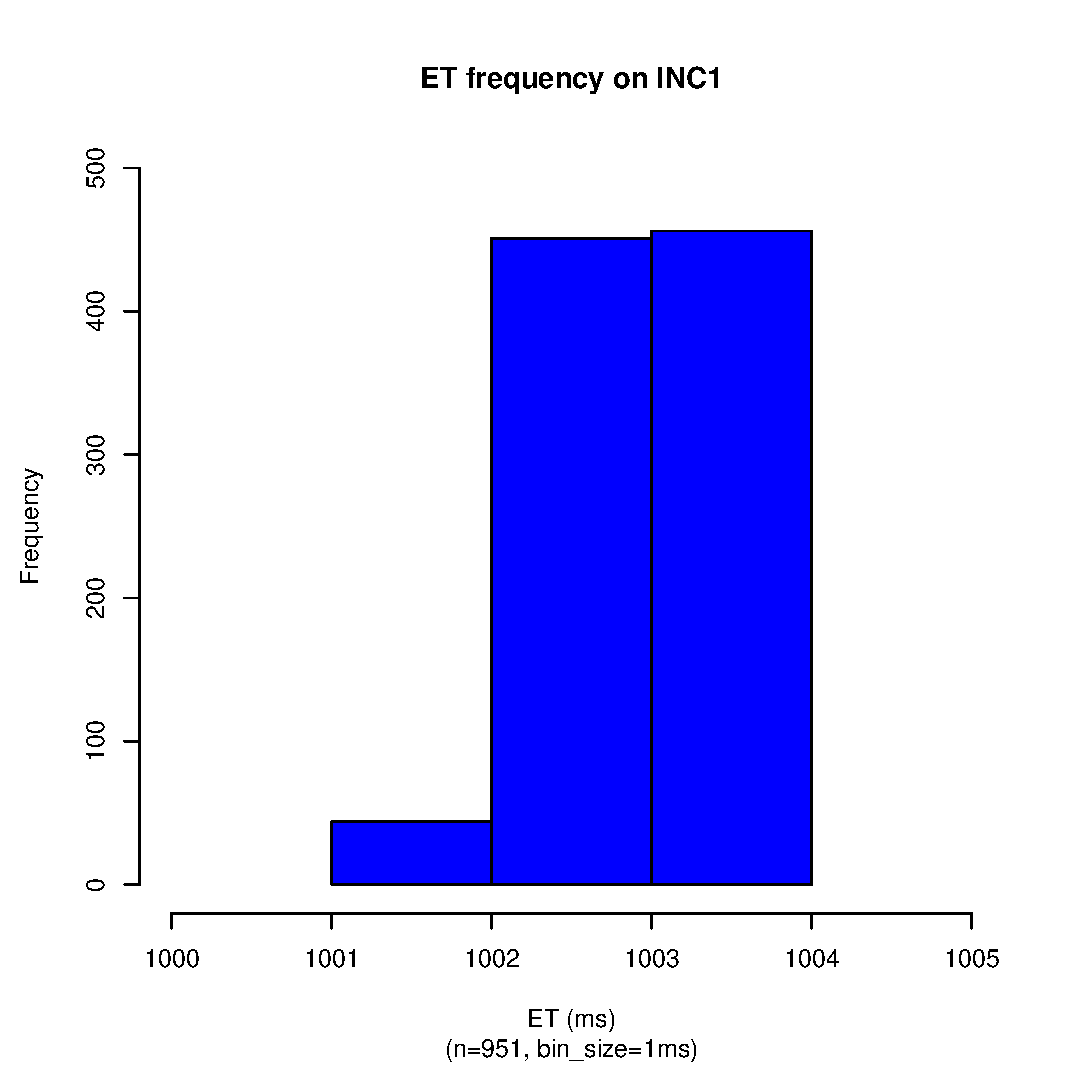
\includegraphics[scale=0.43]{sodb12/1_sec_et_hist_v5.eps}
		\label{fig:s12_inc1_et_hist_v5}
	}
	\subfigure[ET frequency on INC2 on {\tt sodb12}]{
		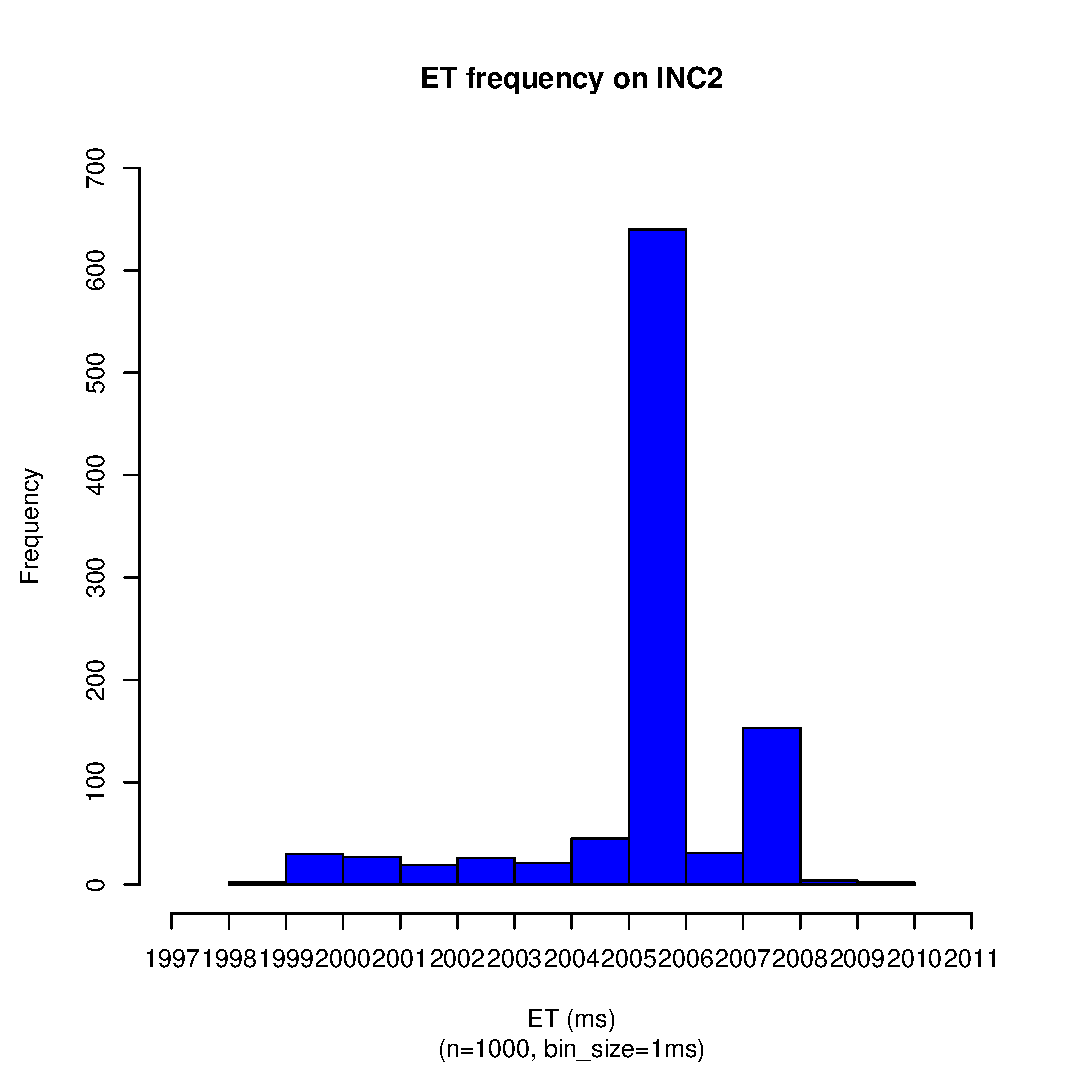
\includegraphics[scale=0.43]{sodb12/2_sec_et_hist_v5.eps}
		\label{fig:s12_inc2_et_hist_v5}
	}
	\subfigure[ET frequency on INC4 on {\tt sodb12}]{
		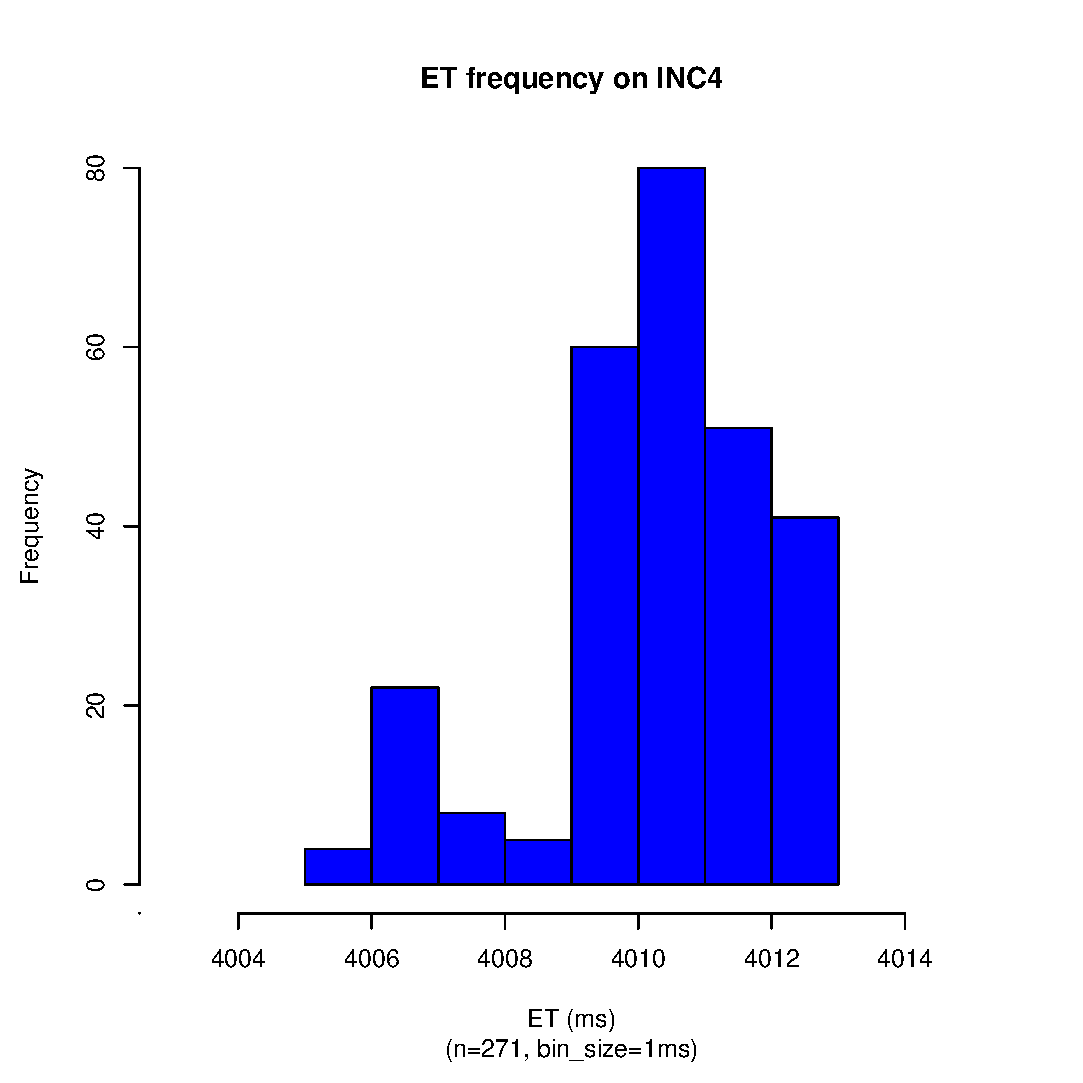
\includegraphics[scale=0.43]{sodb12/4_sec_et_hist_v5.eps}
		\label{fig:s12_inc4_et_hist_v5}
	}
	\subfigure[ET frequency on INC8 on {\tt sodb12}]{
		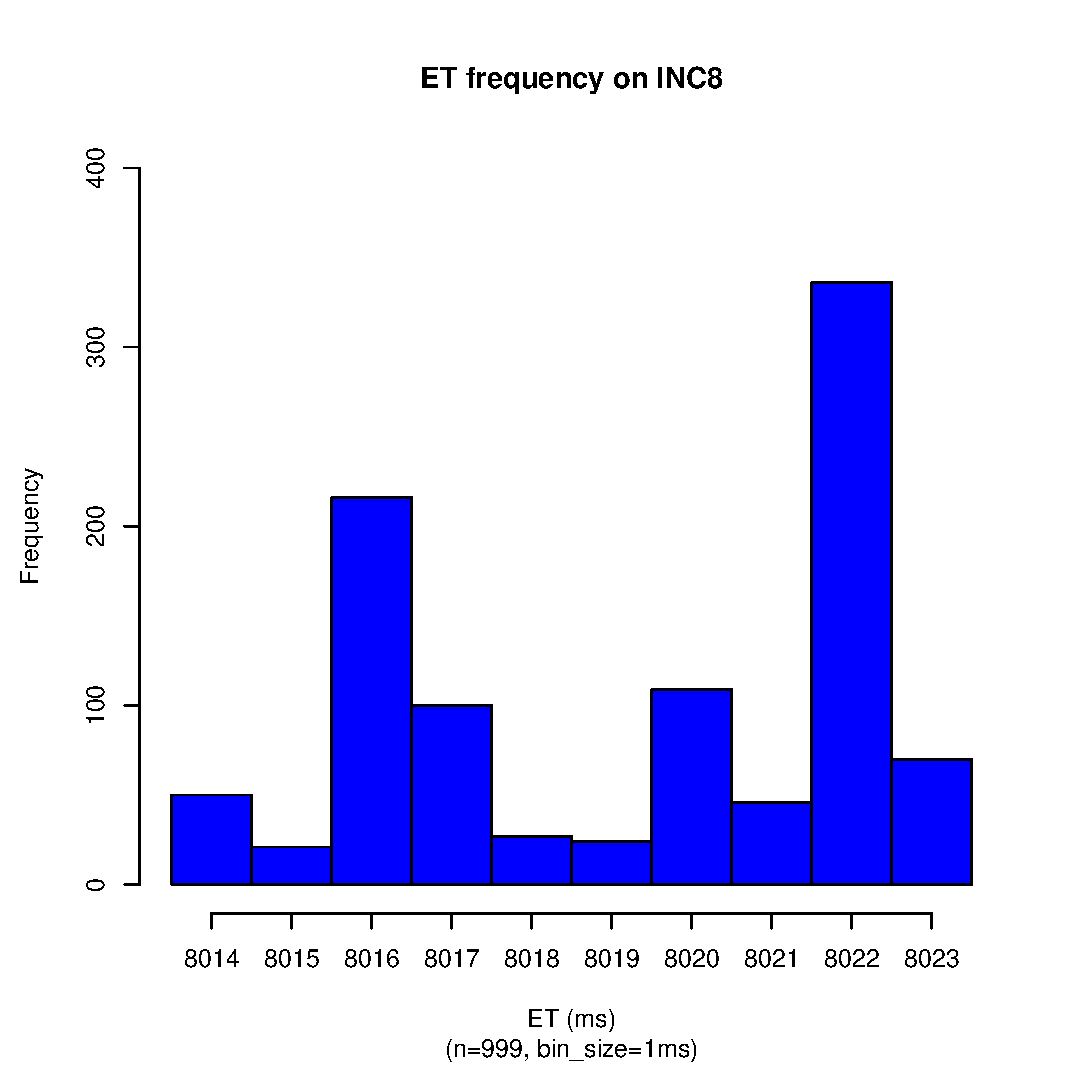
\includegraphics[scale=0.43]{sodb12/8_sec_et_hist_v5.eps}
		\label{fig:s12_inc8_et_hist_v5}
	}
	\caption{ET Histograms of INC1 ... INC8~\label{fig:s12_et_hist1}}
\end{figure}

\begin{figure}[hp!]
	\centering
	\subfigure[ET frequency on INC16 on {\tt sodb12}]{
		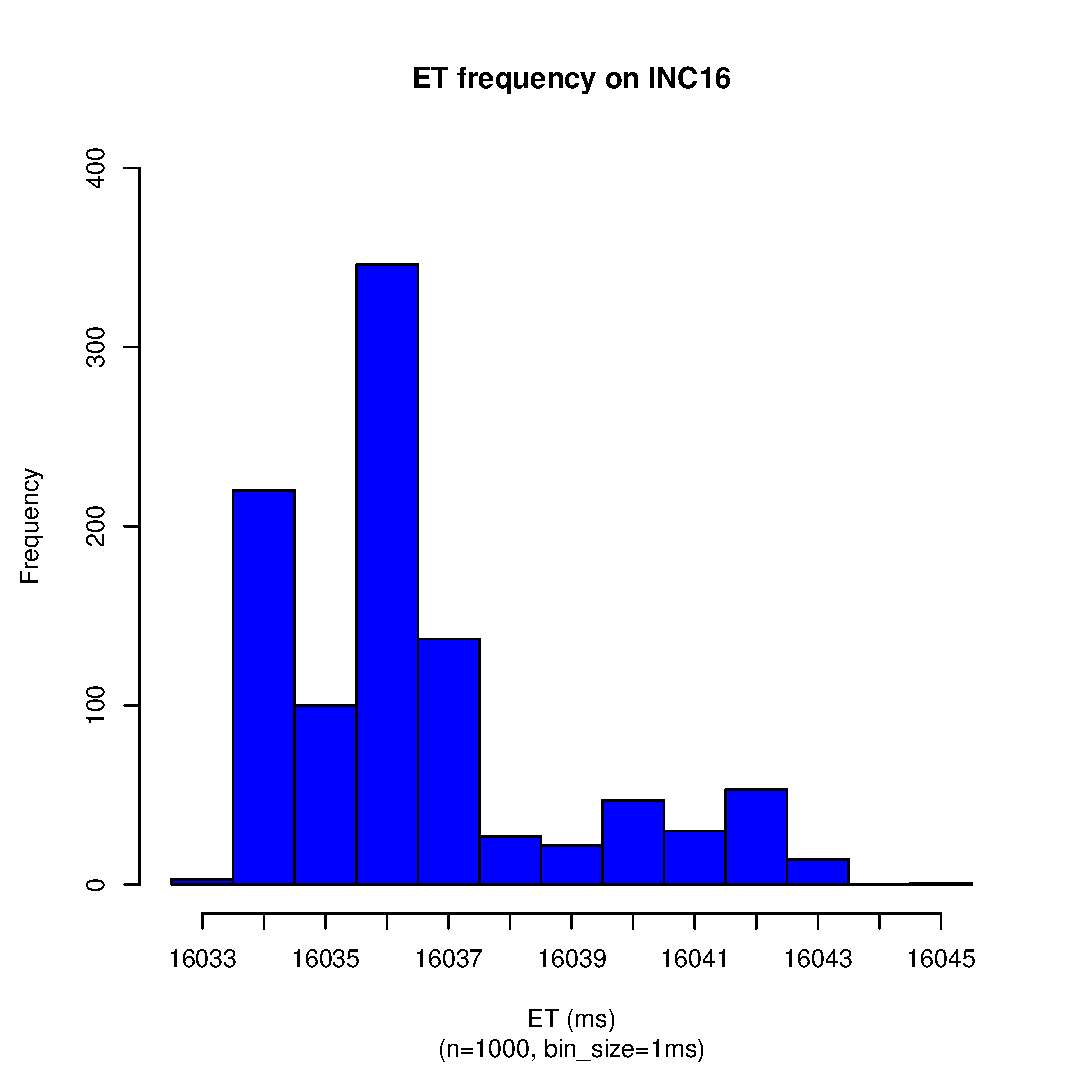
\includegraphics[scale=0.43]{sodb12/16_sec_et_hist_v5.eps}
		\label{fig:s12_inc16_et_hist_v5}
	}
	\subfigure[ET frequency on INC32 on {\tt sodb12}]{
		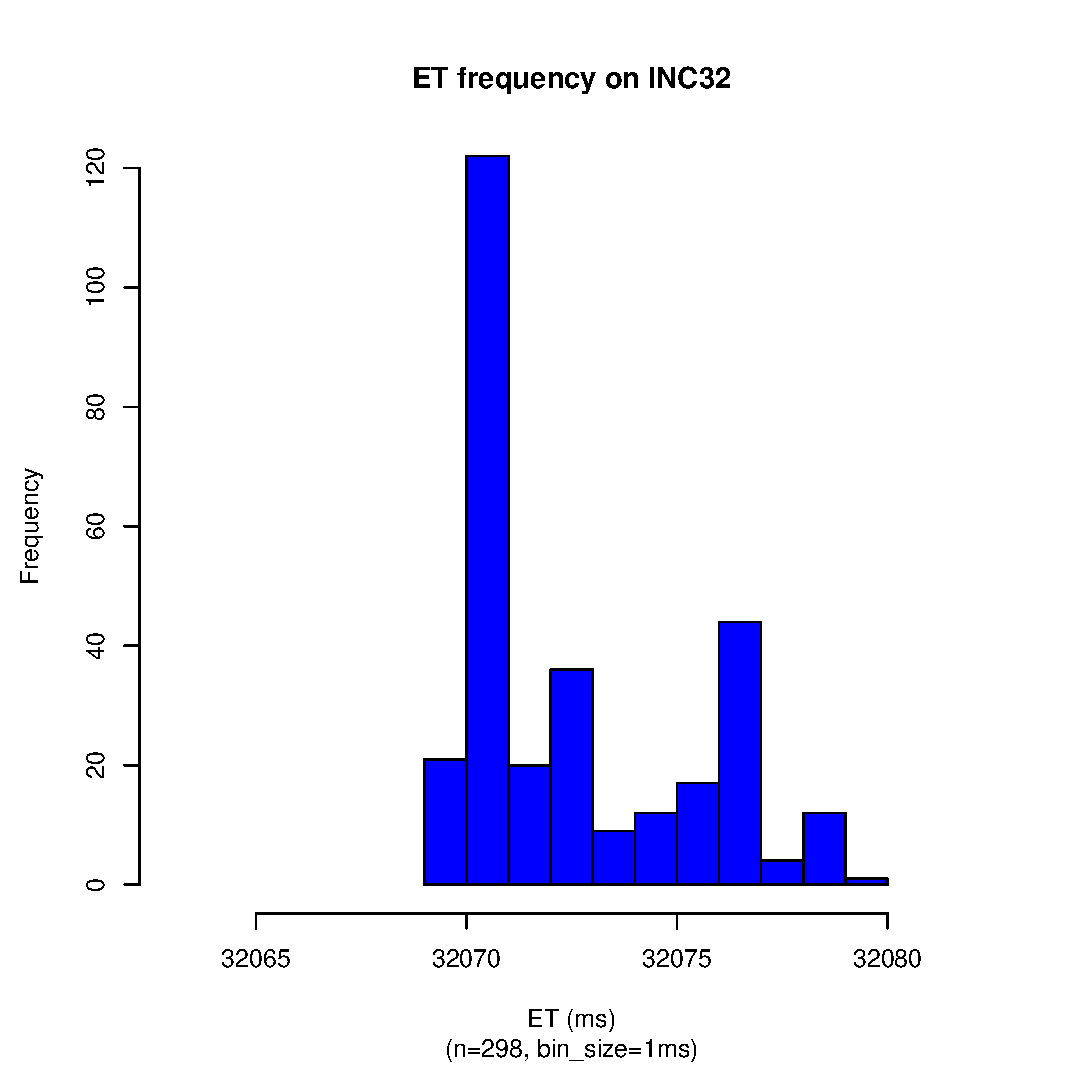
\includegraphics[scale=0.43]{sodb12/32_sec_et_hist_v5.eps}
		\label{fig:s12_inc32_et_hist_v5}
	}
	\subfigure[ET frequency on INC64 on {\tt sodb12}]{
		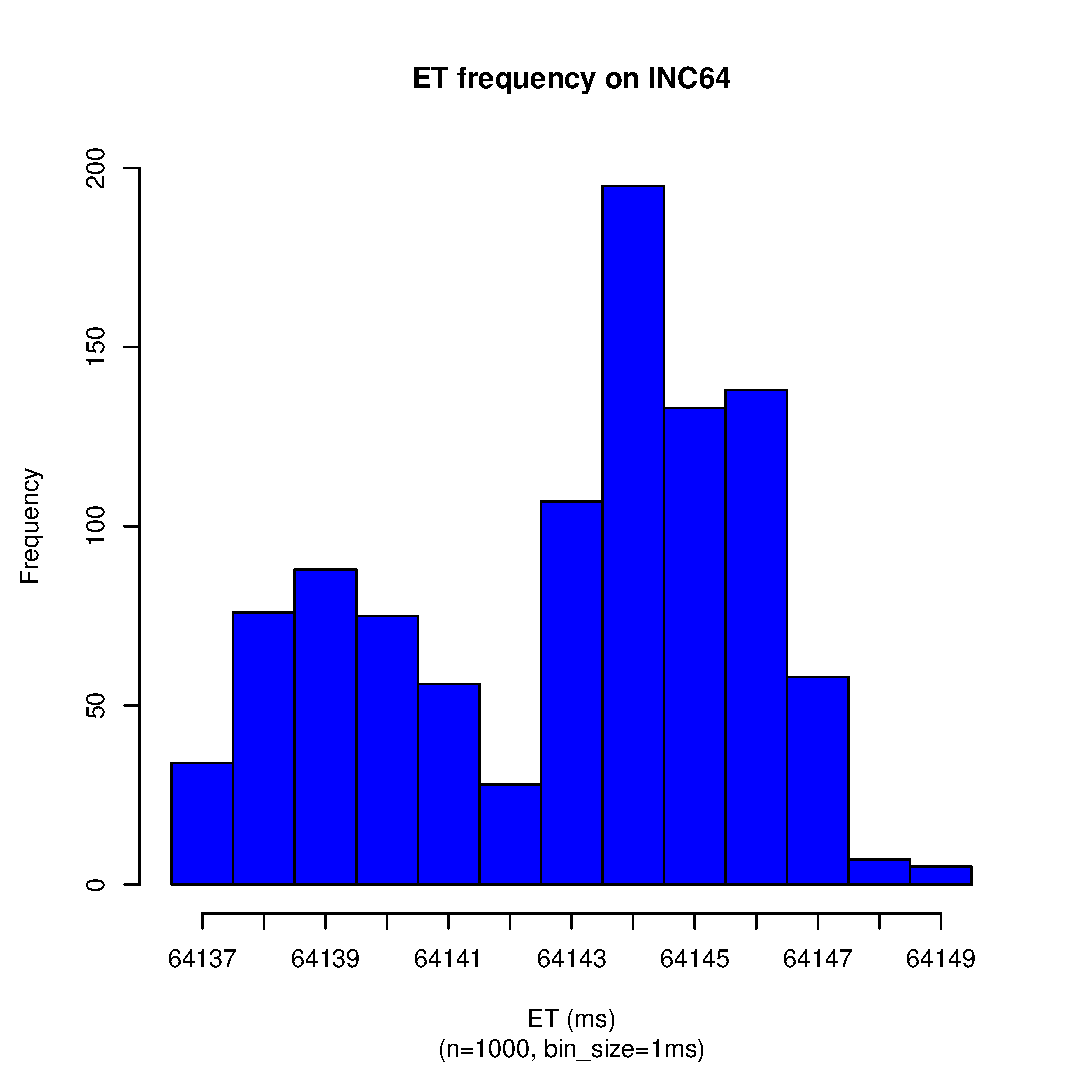
\includegraphics[scale=0.43]{sodb12/64_sec_et_hist_v5.eps}
		\label{fig:s12_inc64_et_hist_v5}
	}
	\subfigure[ET frequency on INC128 on {\tt sodb12}]{
		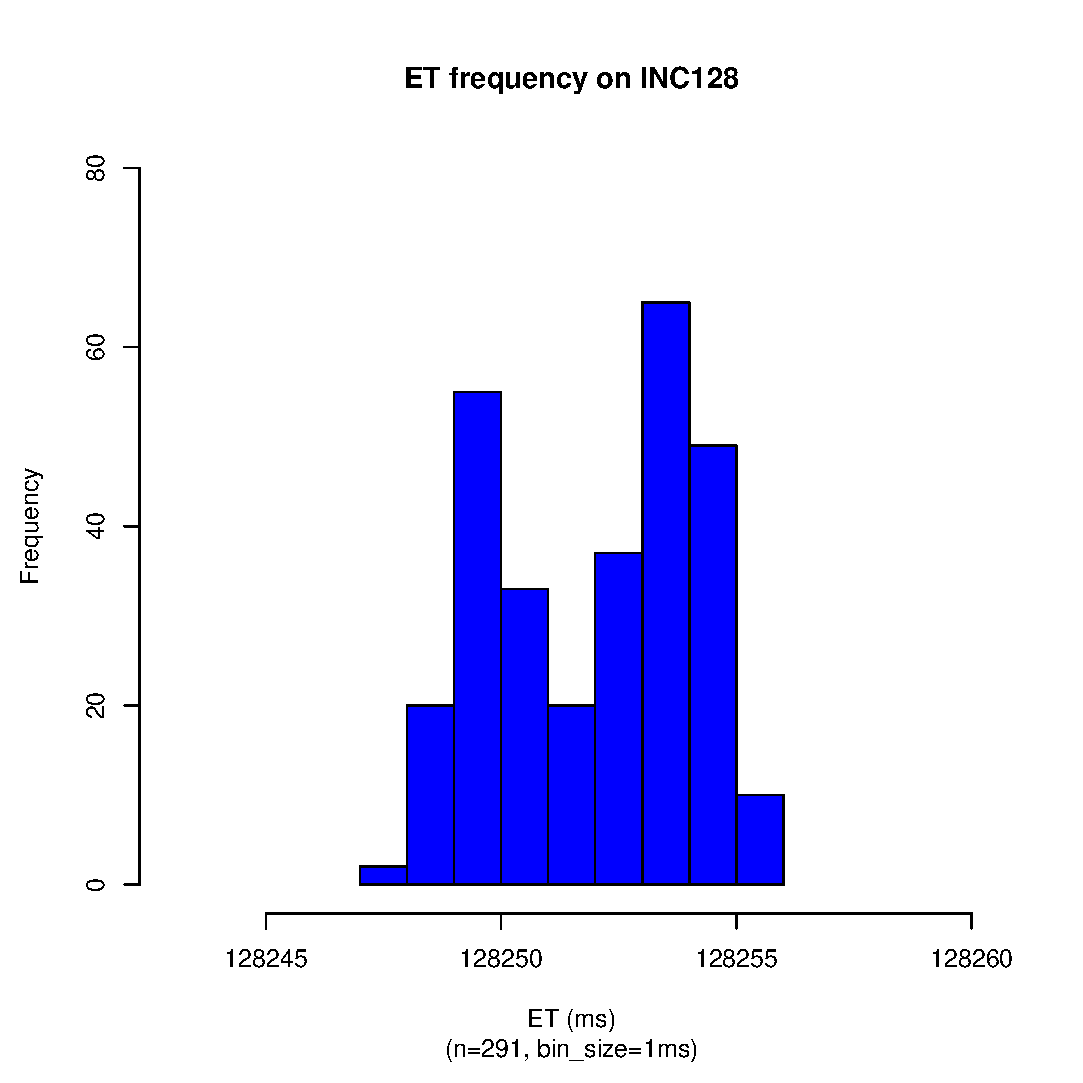
\includegraphics[scale=0.43]{sodb12/128_sec_et_hist_v5.eps}
		\label{fig:s12_inc128_et_hist_v5}
	}
	\caption{ET Histograms of INC16 ... INC128~\label{fig:s12_et_hist2}}
\end{figure}

\newpage

\subsubsection{PT}

\begin{figure}[hp!]
	\centering
	\subfigure[PT frequency on INC1 on {\tt sodb12}]{
		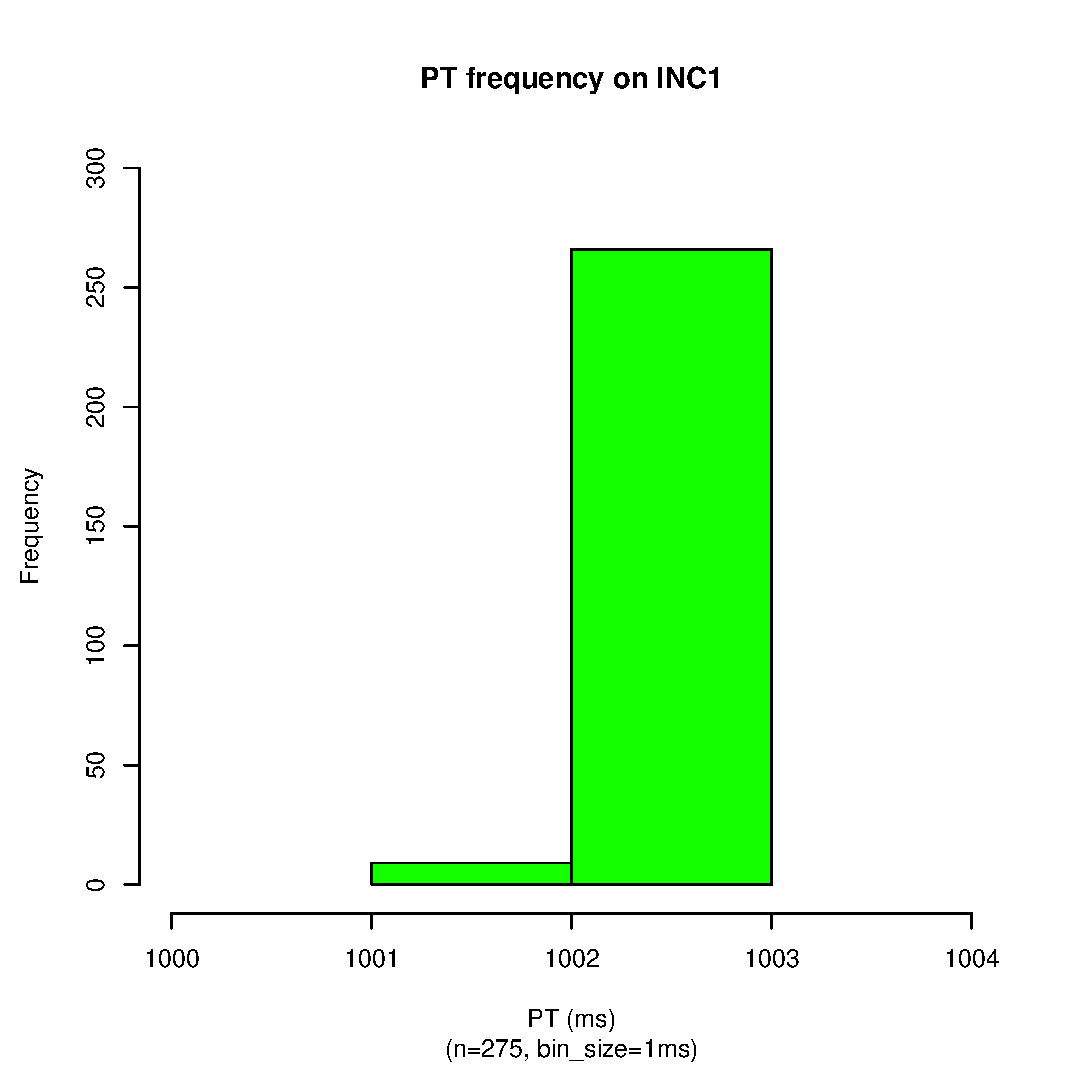
\includegraphics[scale=0.43]{sodb12/1_sec_pt_hist_v5.eps}
		\label{fig:s12_inc1_hist_v5}
	}
	\subfigure[PT frequency on INC2 on {\tt sodb12}]{
		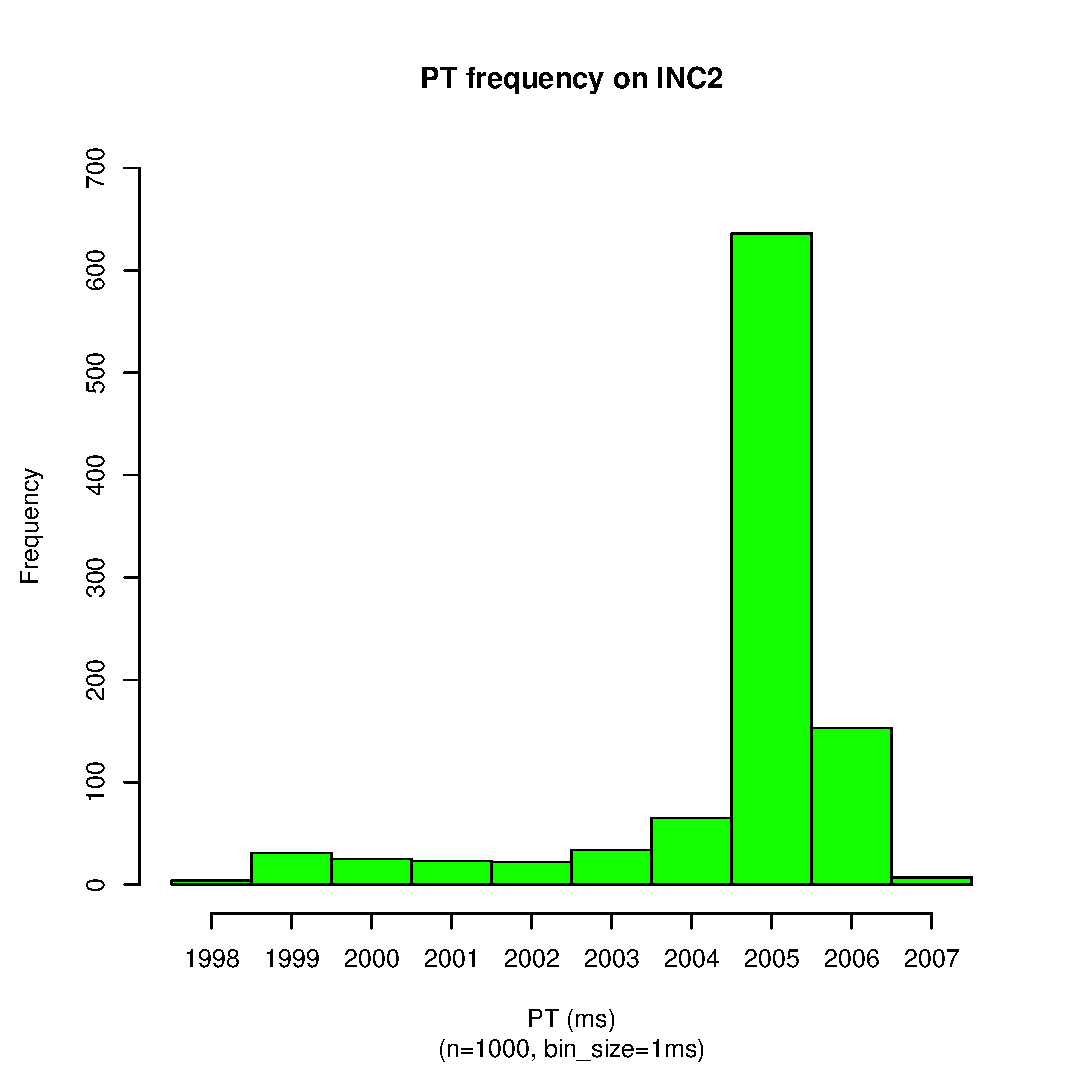
\includegraphics[scale=0.43]{sodb12/2_sec_pt_hist_v5.eps}
		\label{fig:s12_inc2_hist_v5}
	}
	\subfigure[PT frequency on INC4 on {\tt sodb12}]{
		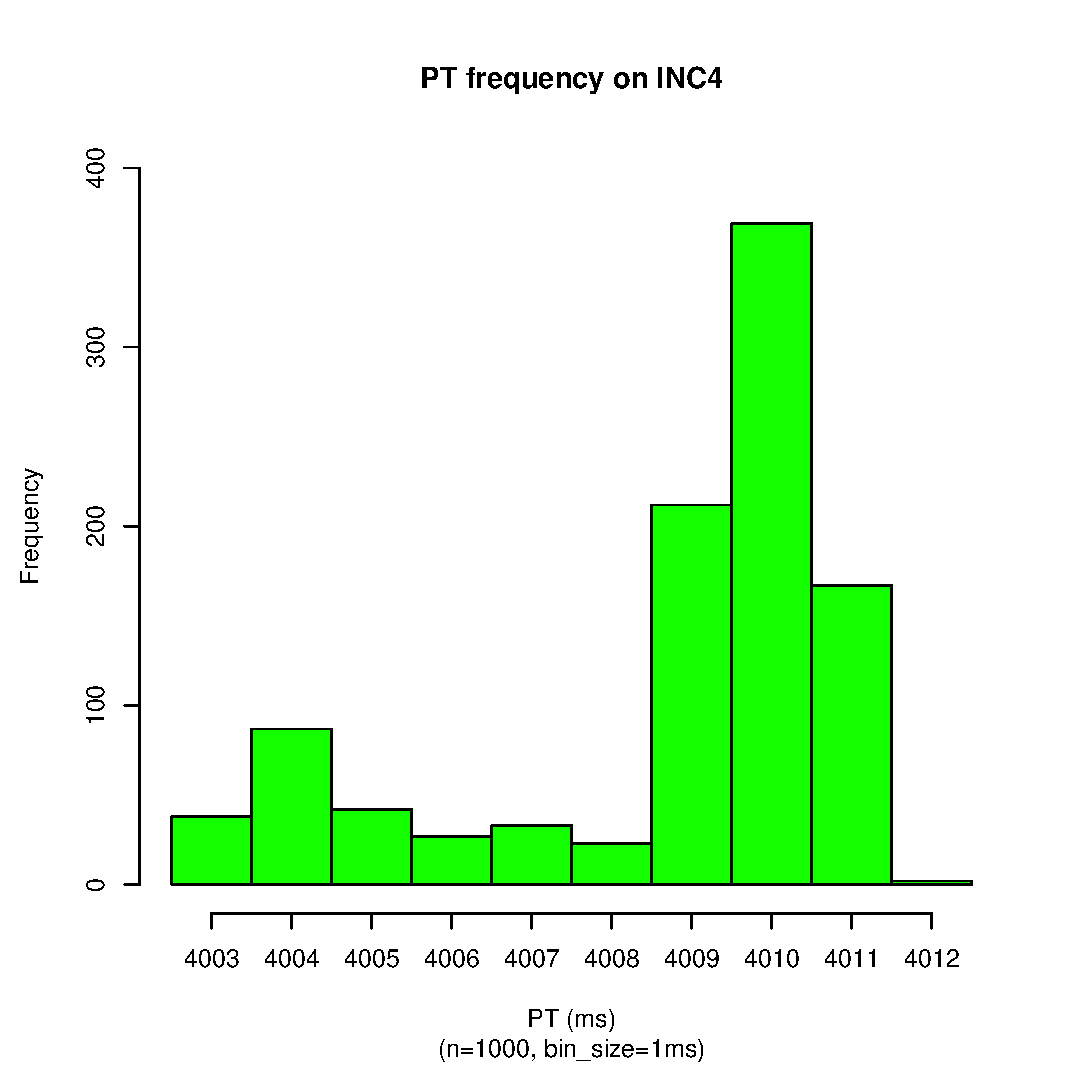
\includegraphics[scale=0.43]{sodb12/4_sec_pt_hist_v5.eps}
		\label{fig:s12_inc4_hist_v5}
	}
	\subfigure[PT frequency on INC8 on {\tt sodb12}]{
		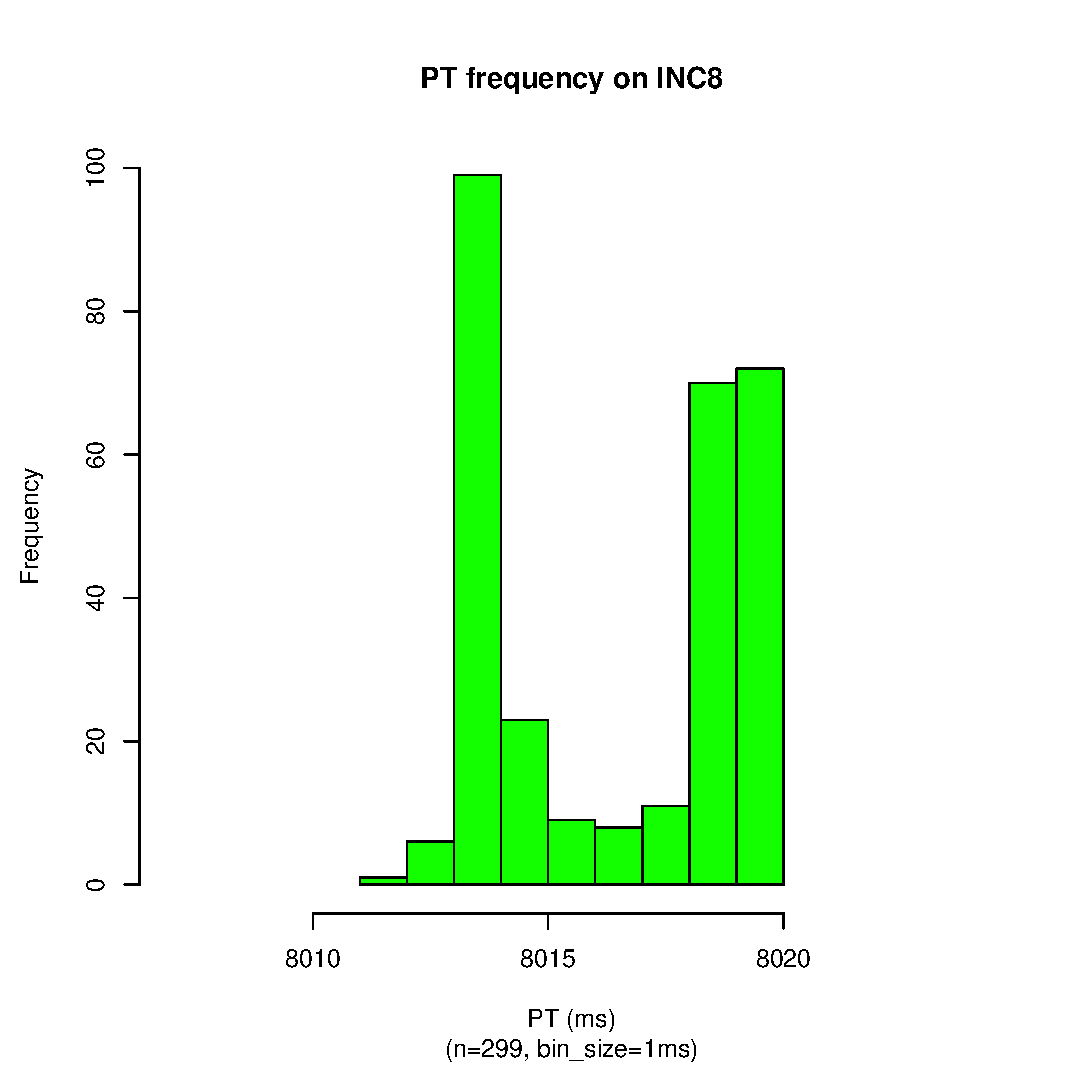
\includegraphics[scale=0.43]{sodb12/8_sec_pt_hist_v5.eps}
		\label{fig:s12_inc8_hist_v5}
	}
	\caption{PT Histograms of INC1 ... INC8~\label{fig:s12_pt_hist1}}
\end{figure}

\begin{figure}[hp!]
	\centering
	\subfigure[PT frequency on INC16 on {\tt sodb12}]{
		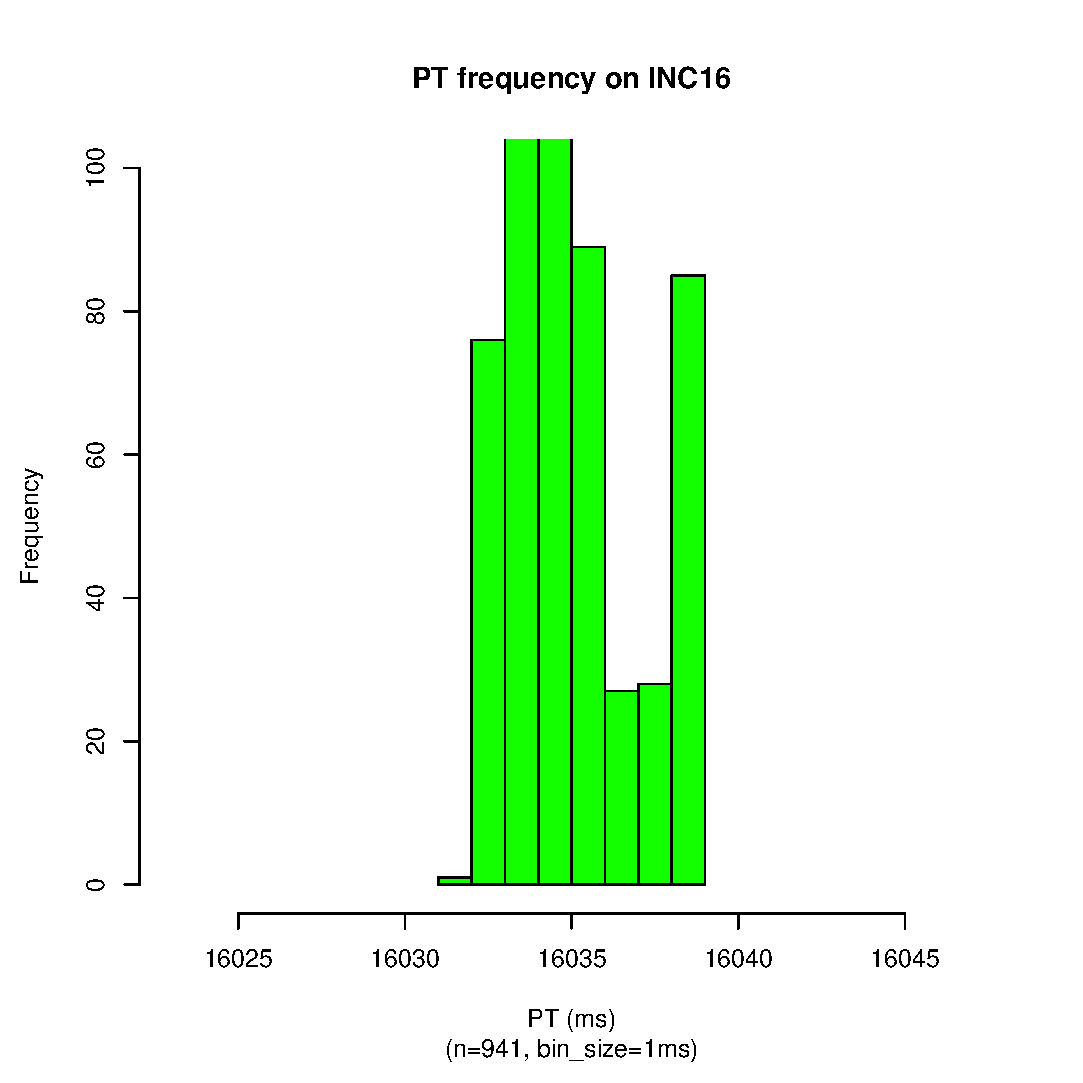
\includegraphics[scale=0.43]{sodb12/16_sec_pt_hist_v5.eps}
		\label{fig:s12_inc16_hist_v5}
	}
	\subfigure[PT frequency on INC32 on {\tt sodb12}]{
		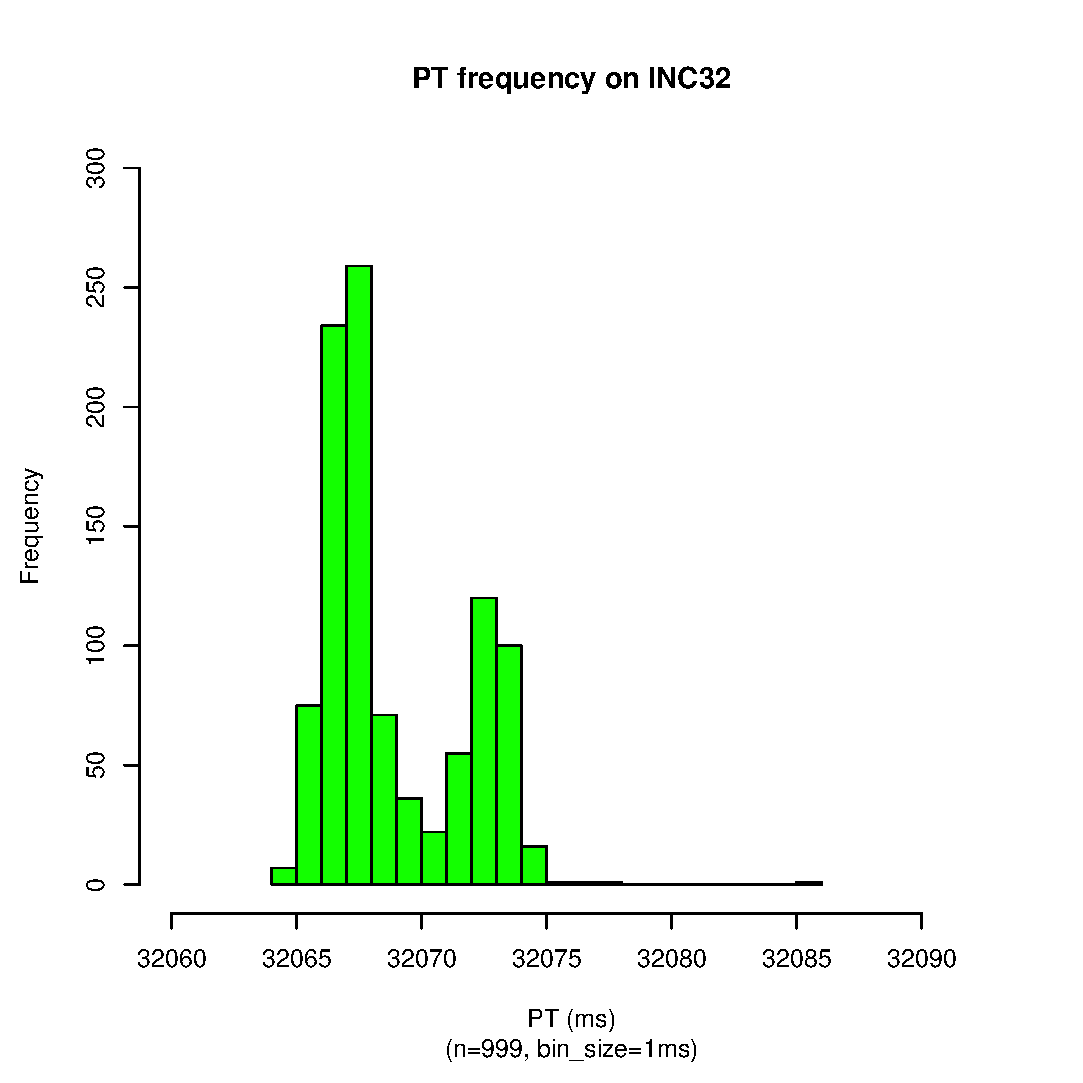
\includegraphics[scale=0.43]{sodb12/32_sec_pt_hist_v5.eps}
		\label{fig:s12_inc32_hist_v5}
	}
	\subfigure[PT frequency on INC64 on {\tt sodb12}]{
		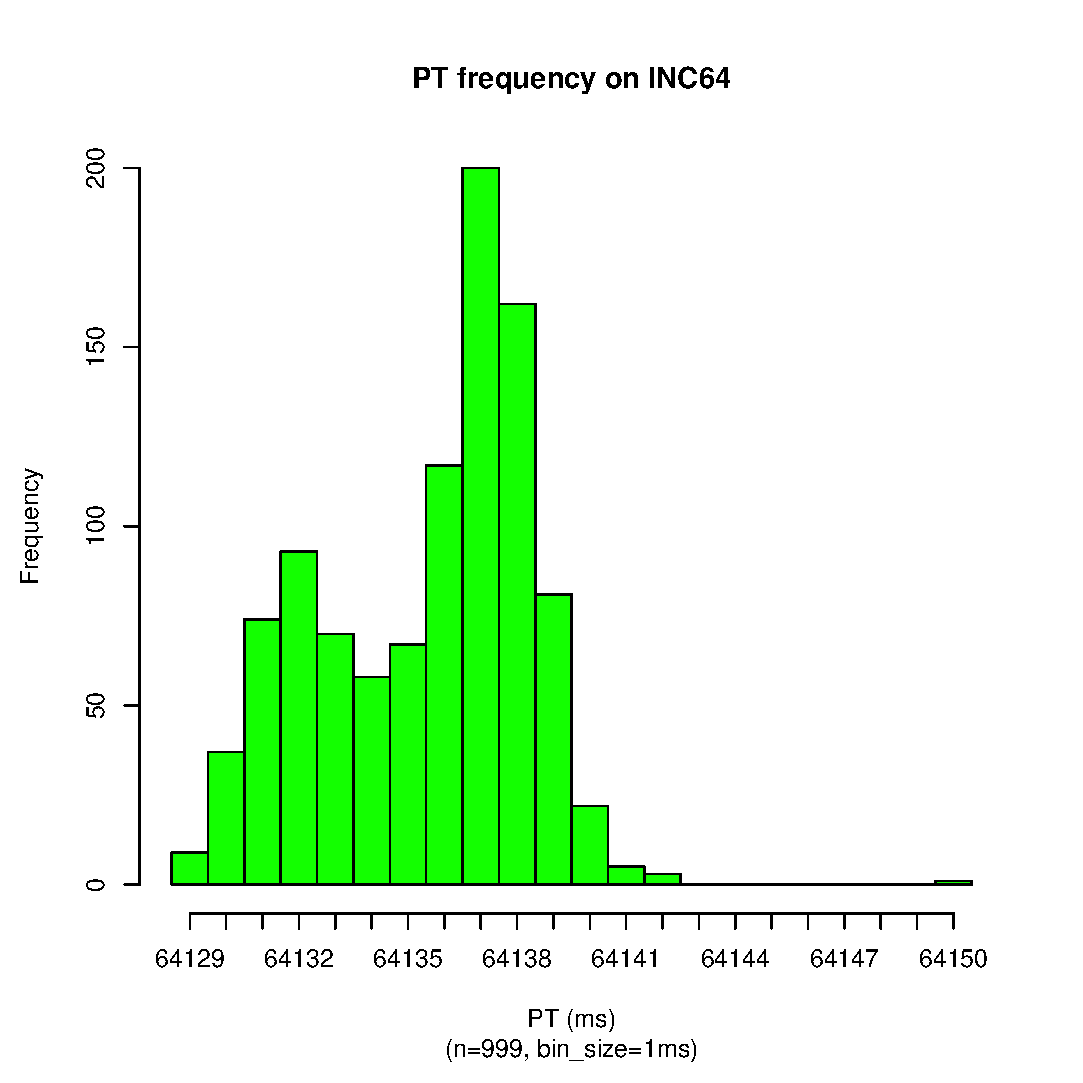
\includegraphics[scale=0.43]{sodb12/64_sec_pt_hist_v5.eps}
		\label{fig:s12_inc64_hist_v5}
	}
	\subfigure[PT frequency on INC128 on {\tt sodb12}]{
		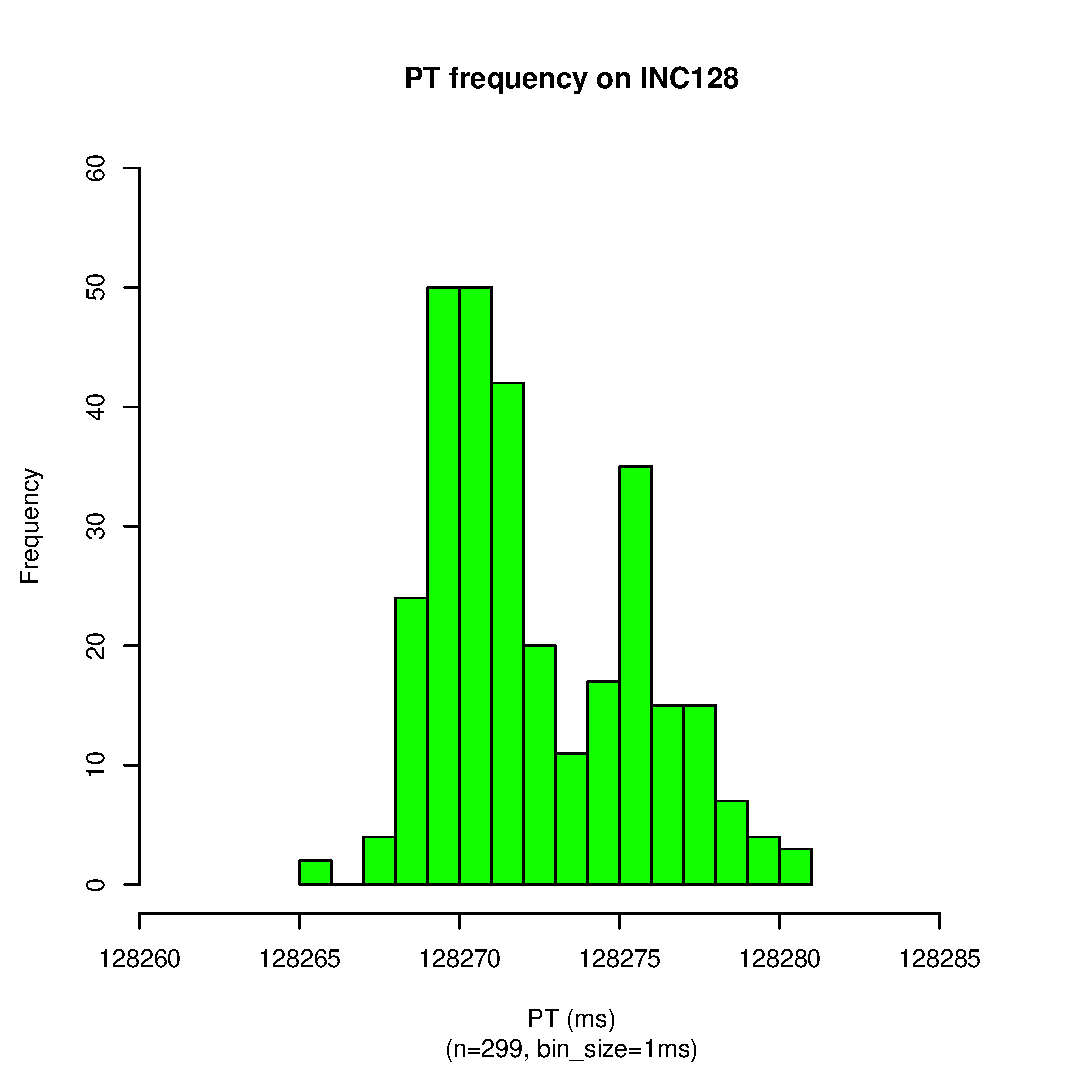
\includegraphics[scale=0.43]{sodb12/128_sec_pt_hist_v5.eps}
		\label{fig:s12_inc128_hist_v5}
	}
	\caption{PT Histograms of INC16 ... INC64~\label{fig:s12_pt_hist2}}
\end{figure}

\end{document}